% File 'gusample.tex' -- Mark Maloof, Michael A. Covington, Isidor Ruderfer
% (Revised 15 December 2010)
% This is an example of how to format a thesis or dissertation using LaTeX 2e
% with 'guthesis.sty' VERSION 3.4 OR LATER.

\documentclass[12pt]{report}

\usepackage{url}
\usepackage[numbers,sort]{natbib}
\usepackage{graphicx}
\usepackage{amsmath}
\usepackage{amssymb}
\usepackage{algorithm}
\usepackage{algorithmic}
\usepackage{svg}

% If there are any other \usepackage commands, put them here.

\usepackage{lib/style/guthesis} % Must be the last package

\newtheorem{theorem}{Theorem}[section]
\newenvironment{proof}[0]{\textit{Proof.}}{}
\newcommand{\qed}{\hfill $\Box$}

% To comment out multiple lines of text.
\long\def\comment#1{}

\title{Peering Through Censorship:\\Tackling Internet Censorship Using P2P Networking}

\author{Eliana V. Troper}

\previousdegree{A.B.}

\thisdegree{Master of Science}  % or Doctor of Philosophy, etc.

\thisdiscipline{Computer Science}

\thesistype{Thesis}     % or Dissertation

% defense or approval date, not today's date...
\thesisday{11}
\thesismonth{April}
\thesisyear{2023}

\professor{Micah Sherr}
%\secondprofessor{Alonzo Church}   % Only if you have 2 major professors!

\fulltitle{Peering Through Censorship: Tackling Internet Censorship Using P2P Networking}

\indexwords{[TODO], Theses~(academic)}

\dean{Alexander Sens}

\memberi{Lisa Singh}
\memberii{Benjamin Ujcich}
% Use \memberiii, \memberiv, \memberv for up to 3 more members if needed.

\begin{document}

\pagenumbering{roman}

\maketitle    % Creates title page, copyright page if any, and approval page.

\begin{abstract}
TODO: Optional for master's thesis but these are nice (max 350 words)
\end{abstract}


\chapter*{Dedication}

TODO: Optional

\pseudochapter{Acknowledgments}

TODO

\tableofcontents

\listoffigures  % Optional - Omit this line if you don't want a list of figures.
\listoftables   % Optional - Omit this line if you don't want a list of tables.

\newpage

\pagenumbering{arabic}  % Ordinary pages have Arabic numerals.

\chapter{Introduction}

People us the internet to communicate and share a variety of content. Some entities choose to censor internet connections. These entities may range from individual network administrators to a full nation-state. In this paper, we explore the state of censorship, existing circumvention sytems, and we design and build a system which tackles several of the limitations present in state of the art systems. [LATER: Add xrefs to sections]

We begin by exploring what we mean by censorship circumvention and establishing baseline terminology for this discipline. We then explore the present theory behind approaches to censorship circumvention. We address the ethics of censorship circumvention as a field, and how the field originated and how that affects the current state of the field.

We then propose several ways to classify existing systems to allow for some comparison between them, and we then explore existing and past systems to understand where the field stands, and where limitations occur. We emphasize systems that are either cutting edge or in active use in the real world.

We also provide an overview of the state of peer to peer (P2P) networking, focusing on succesful project operating in the real world. We provide a deeper dive into the Interplanetary File System (IPFS) and the underlying networking library, LibP2P. These programs are used extensively in out proposed system.

Having outlined what is and has succeeded in censorship circumvention in both the real world and theory, we propose a system that addresses the flaws of the current cutting edge systems. We call this system CN. [TODO: fn code name] We discuss the architecture of this system, putting a particular emphasis on the underlying data structure and network topology.

We build this system and build a benchmarking tool and other apps on top of this system. We use this benchmarking tool to show that the system functions with strong performance. We then begin to simulate a censor based upon theoretical and real world adversaries, and then benchmark the system again, showing that even under severely censored circumstances, we are able to maintain [adequate/good/strong] performance. We also explore what regions of the world would have to operate in more censored circumstances at present.

We then conclude and offer some opportunities for future work.

\chapter{Background}

The term censorship has taken on a life of it's own in the modern social and political context. We are \emph{not} exploring the general connotation of censorship, rather, we are exploring a specific type of censorship that existing in a networking (particularly internetworking) context. We will explore some key concepts and present a short model of networking.

\section{Networking concepts}

We are going to consider the internet as it currently exists, rather than historical states of the internet. Some key concepts:

\begin{itemize}
  \item Internet Protocol (IP) addresses: These are used to represent endpoints of a connection, and are used for routing. Within a network, other identifiers, such as MAC addresses, are used for routing, however, we are focused on routing between networks and will only consider IP based routing as we explore censorship circumvention. We will use IPv4 addresses throughout as sample addresses, though conceptually IPv6 addresses function similarly for the focuses of this paper.
  \item Domain Name System (DNS): DNS resolution is used to map from human-readable and memorizable addresses that map to IP addresses (e.g. georgetown.edu resolved to 23.185.0.2 at the time of writing). [TODO: Explore the transparency of these, DNSSEC, etc]
  \item Router: Routers perform routing for networking, as well as other functions that act on network traffic. They may be the home of a NAT, a firewall, or censorship software. The controller of a router may access and manipulate any traffic which passes through it.
  \item Firewalls: These are software that may restrict traffic based on rules. These rules may be simple or complex. These have positive uses, such as securing a network from attacks.
  \item Network address translation (NAT): A NAT is used to map network addresses seen on one side of a router to those seen on the other side of a router. These are frequently used to house potentially thousands of devices behind a single internet facing IP address. Most humans use devices located behind a NAT.
\end{itemize}

\begin{figure}
\begin{center}
{\includesvg{figures/networking}}
\end{center}
\caption{A model of networking, sufficient for exploring censorship circumvention [TODO: Add final arrows, some sample traffic]}
\end{figure}

\section{What is censorship circumvention?}

When we discuss the subfield of censorship circumvention when discussing networking and security, we are \emph{not} discussing all forms of censorship that a web user might face - we are discussing censorship on-the-wire of active internet traffic, which usually consists of blocking access to specific services. We do not consider a service blocking certain conduct (e.g. a social network restricting hate speech) the censorship that we are circumventing. We aim to allow a use to connect to any service they would like (notwithstanding technical limitations) - not to allow a user to use any service how they would like. Throughout this paper, when we mention censorship, we mean on-the-wire censorship of reaching services.

\subsection{Ethics}

We recognize that some users run heinous services on the web - most of which are illegal in any existing jurisdiction. We believe that the best approach for ceasing access to these heinous services is best done through a legal system - ie, investigating and identifying the perpetrator(s), turning off the service directly, and prosecuting any perpetrator(s) of said acts. We note that most morally reprehensible acts that are frequently associated with anonymity and censorship circumvention systems involve actions that occur in the real world (e.g. exploitation of children, weapon/drug/human trafficking all involve actions that occur in the real world either prior to distribution on the internet or triggered by actions on the internet).

The only notable class of crime which can occur without physical, real-world actions is piracy/IP violations. We believe that targetted legal actions (e.g. DMCA takedowns) can mitigate the issue, and that the cost of further mitigation through censorship would lead to large collateral damage of legal content and a chilling effect of legal speech and usage of the web, and as such the possibility of a circumvention system being used for piracy/IP violations is an acceptable risk given the ability to mitigate damage through the legal system.

\subsection{Threat model and adversary}

Censorship circumvention is an abstract concept, and approaching it in a scientific way requires properly defining and scoping the task. We have already defined the task, [TODO: xref] and must now scope the problem. We will scope our problem by creating a \textbf{threat model} of the censor we are aiming to thwart, termed \textbf{the adversary}.

An adversary has an \textbf{area of influence}. This is an area an adversary controls the network of, and can control (either directly or through compulsion) any service providers within. We assume an adversary may have an area of influcence consisting of several nations, with at least one nation outside of the area of influence of \emph{any} censor.\footnote{This does not mean that this nation does not have the technical capability to censor, but rather does not perform any censorship either directly or via threatening a start of censorship.}

Our adversary has effectively infinite resources, but is bound by the laws of physics and as such is bounded by the difficulty of computational problems (and the known solutions to these problems, e.g. even if P=NP, the solution is not known, and as such cannot be used). These resources may include labor, capital, technical expertise, and total control of the legal system.

We also assume that our adversary has access to the source code of any circumvention system available, and knowledge of the existence of our circumvention system. We discuss why security through obscurity cannot be used in an effective circumvention system in [TODO: xref].

We also assume that our adversary only takes actions \textbf{on-the-wire} and at \textbf{service providers} within their area of influence - effectively, the adversary isn't interested in any individual in particular and is performing a dragnet operation, rather than an operation targetting a specific entity. We can use a thought experiment to justify this: if an adversary had a person looking over your shoulder or using video surveillance, they could simply look at what you are doing and punish you directly, no need to expend the resources needed to censor the web.

We assume our adversary has some interest in the utility of the internet and certain technologies on the internet. This means two things: an adversary will not shut down the internet in it's entirety\footnote{Internet shutdowns are a trivial way to censor forbidden internet usage - at the expense of shutting down any non-forbidden usage. [TODO: Discuss prior shut downs in another section and xref]} and an adversary has some threshold of unacceptable collateral damage caused by potential censorship techniques.\footnote{Similar to a full internet shutdown, if an adversary wanted to block all access to a specific HTTP site, they could block \emph{all} HTTP traffic, at the expense of blocking every HTTP site. This piecemeal web censorship could even be thwarted with a circumvention system that simply proxies HTTP traffic outside of the area of influence within an unblocked protocol and connects to HTTP sites from outside the area of influcence. This starts to show that any non-complete shutdown of internet traffic may have gaps for circumvention techniques. We discuss collateral damage further in [TODO: xref].}

Finally, we note that any technique that subverts this adversary will also work when weakening the strength of these assumptions - e.g. if the adversary controls one nation instead of several, we have more area to run a circumvention system from; if the adversary is only willing to take actions at service providers and not on-the-wire, anything that can thwart an adversary that takes both actions could trivially thwart the adversary that only performs actions at one. We also note that a system could detect the type of actions an adversary is taking and maximize performance based upon what subset of possible actions an adversary is taking - e.g. an adversary that is not touching services leaves an easy path for a circumvention system to use - those services themself.

[TODO: Basic model + adversary]

\begin{figure}
\begin{center}
{\includesvg{figures/networking}}
\end{center}
\caption{A model of networking, with our adversary model overlaid [TODO: Once networking diagram is finalized, add an adversary]}
\end{figure}

\subsection{History and basics}

The web arose in a relatively haphazard fashion [TODO: discuss a bit more]. The web was not a place where adversaries engaged in censorship (if they paid any mind to the web whatsoever). Instead, as the web became more prominent and more global, individuals realized that they could be tracked, and that they desired anonymity. This led to the development of basic and advanced anonymity software, with proxying being a basic tool for this and Tor being the most prominent example of full fledged anonymity software.

As this occurred, the web continued to grow in prominence, and the concept of "Web 2.0" arose - regular users could post content to sites such as message boards and social media sites. People could organize quickly and effectively across larger distances and with people they had never met in the past. Governments took notice - and censorship began.\footnote{The main justifications censors employ are maintaining law and order, preventing the spread of disinformation, preventing access to "unwholesome" content, or economic protectionism. [TODO: Would be cool to cite one or several instances of these justifications coming from the horses mouth]}

When internet censorship arose, basic techniques were used. These include:
\begin{itemize}
  \item Blocking specific IPs: Traffic to or from various IP addresses could be dropped. This is simple and low cost.
  \item Blocking DNS resolution: DNS resolution traffic for specific requests could be dropped (or replaced). This is simple and low cost. [TODO: address DNS encryption and authentication]
  \item Legal mechanisms: If a service exists within the area an adversary controls, they could simply take down the service itself. Since we define the adversary to not control the whole world, we will ignore this form of censorship throughout this paper, as a restricted service could avoid this by relocating out of the sphere of influence of an adversary.
\end{itemize}
These techniques are sufficient to cut off access to services for users who are either unaware of a censor, unaware that circumvention is possible, users who do not care about the actions of a censor, or out of laziness. A user would have to actively use something that circumvents these simple blocks. The solution to avoid IP blocking and censoring DNS results is to proxy a users raw traffic outside of a censored area (either through a basic proxy, or something that provides other features, such as Tor). From the view of a censor, a user would not be accessing a restricted service, they would be accessing a proxy service.

\begin{figure}
\begin{center}
{\includesvg{figures/networking}}
\end{center}
\caption{A model of networking, with our adversary performing basic censorship [TODO: Once networking diagram is finalized, show blocking]}
\end{figure}

Censorship circumvention arose as a by-product of tools made for purposes that were not focused on censorship circumvention. As primitive censorship began, people realized that anonymity software such as Tor or even a basic proxy could be used to access services that would otherwise be blocked. The entrances to these proxy services and Tor were accessed via well known IP addresses or DNS names.\footnote{The reason these were well known is that, if you want the public to access your service, they must know how to access these services, including the addresses of your service. These must be made public to allow people to access your service. A censor has access to public information.} Censors began being blocking access to these services, in additon to their original censorship targets. This set off a "censorship arms race."

At this point, those who used and built the anonymity software recognized that censorship circumvention would be crucial for maintaining access to these tools, and others realized that censorship circumvention in-and-of itself would be useful. This effectively led to the rise of a subdiscipline that draws heavily from networking, security, and even game theory, but also exists independently from those subdisciplines, with a variety of stakeholders including governments, NGOs, non-profits, independent programmers, academics, and others interested in developing censorship circumvention techniques. This also leads to a relatively unique feature of this discipline - some techniques were developped in academia, some techniques were developped in the real world, and some were developped in both, and ignoring the results from either thread of research and observation can lead to the development of flawed systems.

\subsection{Current theory of censorship circumvention}

Present censorship circumvention is currently built on two techniques: proxying traffic \emph{out} of the adversaries sphere of influence, and providing access to those proxies. If you can provide access to a proxy, then using existing proxying technology is trivial. The majority of censorship circumvention theory is, therefore, focused on providing access to proxies.

The bedrock of the theory underlying succesful provision of access to proxies is collateral damage.

[TODO: Discuss collateral damage more]

\subsubsection{Modeling collateral damage}

We begin with a basic model - an adversary will engage in the censorship of service $x$ if $B_x - C_x > 0$, where $B_x$ is the average benefit per user of engaging in censorship of service $x$ and $C_x$ is the average cost of engaging in censorship of service $x$. We will refine this formula by switching to a focus on censorship techniques - $(b_{x,1} + b_{x,2} + ... + b_{x,n}) - C_x > 0$, where $b_{x,n}$ is the average benefit per user of censoring service $n$ using method $x$. A censor will engage in any censorhip method where the average benefit reaped by censoring \emph{any} desired services using that method is greater than the cost. Also note that these benefits and costs are based on how they are \emph{perceived} by the censor, not by an objective, bird-eye view of good vs. bad, and they may account for a variety of benefits/cost, including direct financial costs, but also including less tangible value such as "stability".

We now note that each method may only stop a fraction of users accessing a service using a method - so a more realistic formulation would be $(u_{x,1}*b_{x,1} + u_{x,2}*b_{x,2} + ... + u_{x,n}*b_{x,n}) - C_x > 0$, where $u_{x,n}$ is the fraction of users accessing service $n$ that are blocked from accessing service $n$ using method $x$.

We will now break down cost further. $C_x = f_x + m_x$ - where $f_x$ is the fixed cost per user of setting up method $x$ and $m_x$ is the marginal cost of actively engaging in $x$ per user. We will drop $f_x$ from further consideration (ie, $C_x = m_x$) - the cost of setting up a method is a one time cost, and to an adversary with unlimited resources, expending a one time cost averages to $0$ over the long run. We will now explore the marginal cost of $x$. Censorship tools may slow down "good" traffic, and they may erroneously block access to good services. Therefore, $C_x = s_x*i_x + (u_{x,1}*c_{x,1} + u_{x,2}*c_{x,2} + ...  + u_{x,n}*c_{x,n})$, where $c_{x,n}$ is the average cost of blocking service $n$ per user, $u_{x,n}$ is the same as above, $s_x$ is the average fraction of the total value of unblocked traffic retained (due to the reduction in speed caused by enabling method $x$),\footnote{Note that an adversary may engage in multiple stages of filtering, so some subsets of unblocked traffic may experience no slowdown, while some might experience more. For the purposes of our analysis, we can use the average across all allowed traffic.}, and $i_x$ is the value per user of access to all unblocked sites. Combining the above, we see
$(u_{x,1}*b_{x,1} + u_{x,1}*b_{x,2} + ... + u_{x,n}*b_{x,n}) - s_x*i_x + (c_{x,1} + c_{x,2} + ...  + c_{x,n}) > 0$, or, more sucintly:
\begin{equation}
-s_x*i_x + \sum_{s=1}^{n}u_{x,s}*v_{x,s} > 0
\end{equation}
where $v_{x,s} = b_{x,s} - c_{x,s}$.

We could conclude here if a censor engaged in censorship solely using a singular method of censorship - however, censors engage in multiple methods of censorship, and the benefit of succesfully blocking a site is not distributed multiple times if it's blocked by multiple methods, the benefit is only achieved based on new users blocked by a method, or, in short, a singular censorship system $x$ will be implemented if:
\begin{equation}
-s_x*i_x + \sum_{s=1}^{n}\Delta u_{x,s}*v_{x,s} > 0
\end{equation}
Note that all variables are the same, except $i_x$ is now the value per user of access to all unblocked sites prior to enabling censorship system $x$ and $\Delta u_{x,s}$ is the change in the fraction of users who can access service $s$ after enabling $x$.

We have now established an equation used to determine if a censor will enable an individual system, taking existing sytems (or lack thereof) as a given. This is not reflective of reality, where a rational censor will evaluate \emph{all} of their active and potentical circumvention systems in conjunction.

The valuation of a system consisting of censorship systems $1$ through $m$ is as follows:
\begin{equation}
\sum_{x=1}^{m}\sum_{s=1}^{n}\Delta u_{x,s}*v_{x,s} - i_{x} * \prod_{x=1}^{m}s_x
\end{equation}
All variables are the same as previously, except $i_x$ is the value per user of access to all unblocked sites again, $s_x$ is the average fraction of the total value of unblocked traffic retained after enabling all systems $y$ with $0\leq y<x$, and $\Delta  u_{x,s}$ change in fraction of all users blocked using method $x$ that were not already blocked after enabling all systems $y$ with $0\leq y<x$. We will define $x=0$ such that this "censorship" system is the null (non-existent) censorship system, and therefore $s_0 = 1$, and $u_{0,s} = 0$.

We assert that a censor is picking from a number of censorship systems that is small enough such that the censor can evaluate the above equation for every possible set of censorship systems in every permutation such that each set only has one of each censorship system in a reasonable amount of time. [TODO: Maybe justify a bit more?]

A rational censor will enable the set of censorship systems such that the above equation is maximized given every potential set of circumvention systems.

[TODO: Dig into the base rate fallacy]

\section{Prior techniques}

[TODO: Mention parrot is dead]

TODO

[TODO: Mention Tor PTs independently of specific methods]

[TODO: Do mention some things like shadowsocks that are in use but are even further from academics]

[TODO: Mention stego]

\subsection{[Point to point obfuscation]}

TODO

\subsubsection{OBFS and Scramblesuit}

TODO

[TODO: Others]

\subsection{[P2P and P2P-like]}

TODO

\subsubsection{Snowflake}

TODO

[TODO: Iran case study]

\subsubsection{MassBrowser}

TODO

\subsection{High-reliability channels}

TODO

\subsubsection{Domain fronting}

TODO

\subsubsection{Raven}

TODO

\subsection{Decoy routing}

TODO

\section{Real world observations}

TODO

\subsection{Real world vs. academic theory}

TODO

\section{P2P networking}

TODO

\subsection{IPFS}

TODO

\chapter{System design}

We saw that several circumvention systems work given the constraints they were designed for, however, these constraints are either too loose and have known real-world failures under our adversary model, the systems are too difficult to deploy, or they have hit scalability issues.

We propose a system with a clear theoretical backing and acheivable goals based on both theory and real-world observations.

\section{Theory and goals}

First, we want to define system goal and highlight some non-goals that are close to censorship circumvention, but are not directly used for them.

We aim to thwart the adversary we outline in [xref]. We will rely heavily on the concept of collateral damage. [TODO: Discuss collateral damage further]

We are \emph{not} aiming to provide anonymity.\footnote{Perhaps our system could be used to access an anonymity system, but we do not want to guarentee anonymity or guarentee that the system will not leak information that may break anonymity, though we are not delibrately trying to break anonymity, we are also not evaluating our system for it at this point.} We feel the need to emphasize this, as most current systems that are functional in the real world are used as pluggable transports by Tor.\footnote{Our system could be used as a PT, as we do have a golang implementation, however, evaluating this system for usage as a PT is reserved for future work.}

\subsection{Comparing existing systems}

Earlier, [TODO: xref] we discussed a variety of censorship circumvention systems. Observing how and why each of these work, and the drawbacks associated with each of them will allow us to formulate goals we wish to acheive and working techniques we may use. We present a short summary of previous systems in [TODO: xref table], comparing and contrasting their succesful techniques and transports, and their individual drawbacks.

\begin{table}
\caption{Comparison of existing systems.}
\begin{center}
[TODO: Make table take whole page sideways, make in latex when finalized]
\makebox[\textwidth]{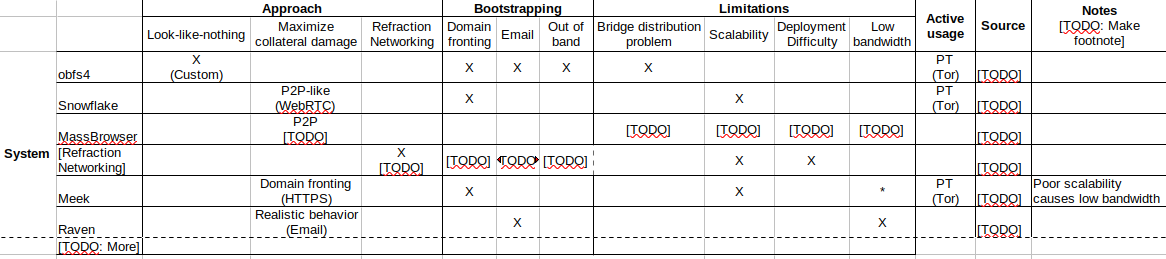
\includegraphics[width=\paperwidth]{tables/comparison-draft.png}}
\end{center}
\end{table}

We see that existing systems are limited by at least one of the following:
\begin{itemize}
  \item The bridge distribution problem [TODO: Xref]
  \item Scalability
  \item Deployment difficulty
  \item Low bandwidth
\end{itemize}

Another key observation is that \emph{collateral damage} is the bedrock of the theory behind a circumvention system - as such, any system must be based around maximizing this - the ideal system will make the only feasible way to shut down the system effectively shutting down a large portion of internet traffic. 

[TODO: Discuss false positives + the overhead of blocking traffic]

[TODO: More]

We also note that existing systems require a user to download and use specialized software, and that systems usually require using anonymity software such as Tor to reap the benefits of censorship circuvmention. While anonymity is a useful [thing] to have in some circumstances on the web, getting the drawbacks of common anonymity software [TODO: outline] is not ideal.

\section{Implementation}

TODO

\chapter{System evaluation}

TODO

\section{Performance}

TODO

\section{Bootstrapping availability}

TODO

\chapter{Conclusion}

TODO

\section{Future work}

TODO

\appendices  % Indicates that appendices follow.
% If there's only one, use \appendix instead.

\chapter{Sample appendix}
SAMPLE
\section{Sample section}
SAMPLE

\chapter{Second sample appendix}
SAMPLE


\bibliographystyle{plain}
\bibliography{lib/cites}

\end{document}

